\chapter{Le framework Mechanics, Dynamics, Aesthetics}

La conception de jeu est le processus de réflexion nécessaire à la création d'un jeu vidéo ou de n'importe quelle sorte de jeu. C'est le chemin que suit le jeu depuis une idée jusqu'à sa réalisation. De nombreuses étapes permettent de mettre en place tous les aspects du jeu pour le mener à sa version jouable. La mise en place du monde dans lequel le joueur évoluera, les règles qu'il devra suivre pour avancer, les éléments graphiques qu'il rencontrera tout cela est définit lors de la conception. Le jeu vidéo est cependant difficile à concevoir et surtout à documenter. Un logiciel classique répond au besoin d'un utilisateur qui s'en sert pour résoudre une problématique. Un jeu quant à lui doit apporter un but au le joueur, l'envie de continuer à l'utiliser et de générer des émotions pour être apprécié. Il est très compliqué de définir une méthodologie précise pour décrire une émotion générée ainsi que tous les éléments techniques autour d'un jeu vidéo. C'est ce que le Framework \gls{mda} propose.


\section{Le jeu : un échange entre \emph{Game Designer} et Joueur}
Un \emph{Game Designer} créé un jeu dans le but de générer une expérience de jeu. Cependant l'utilisation que le joueur fera du produit finit est impévisible \cite{MDA_formal}. Dans leur article Hunicke, LeBlanc et Zubek \cite{MDA_formal} découpent un jeu en trois aspects distincts : les règles, le systéme et le \guillemotleft fun \guillemotright. Ces trois aspects sont à l'origine des trois parties du Framework MDA comme indiqués dans la Figure \ref{fig:mda}.
\begin{figure}[H]
    \begin{center}
    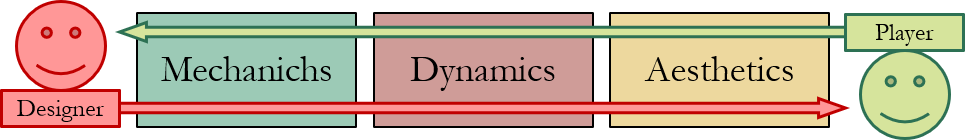
\includegraphics[width=14cm]{10_img/chap3/mda.png} 
    \caption{Contenu des parties du Framework MDA \cite{MDA_formal}}
    \label{fig:mda}
    \end{center}
\end{figure}


%MDA: A Formal Approach to Game Design and Game Research Robin Hunicke, Marc LeBlanc, Robert Zubek
%A better recipe for game jams: using the Mechanics Dynamics Aesthetics framework for planning Paris Buttfield-Addison,Jon Manning,Tim Nugent
%\Design, Dynamics, Experience (DDE): An Advancement of the MDA Framework for Game Design
\section{\emph{Mechanics}}
Les \emph{Mechanics} du jeu sont tous les éléments composant le jeu au niveau de la représentation des données et des algorithmes. Les éléments sont dans des catégories qui permettent non seulement de les classer mais également d'aider à les définir plus précisément. Ces catégories peuvent comprendre des attributs et des spécificités qui sont appliquées aux éléments contenus dans les catégories.

Les \emph{Mechanics} comprennent également les actions, comportements et mécanismes de contrôles mis à disposition du joueur. Cela peut correspondre aux mouvements d'un personnages, aux actions possibles sur des objets ou aux interactions entre les objets. Les règles sont aussi définies dans les mécaniques.


\section{\emph{Dynamics}}

Les \emph{Dynamics} sont les conséquences des \emph{Mechanics}. Elles décrivent le comportement de l'exécution des \emph{Mechanics} lorsqu'elles seront utilisées par le joueur \cite{GAMA_MDA}. Ces \emph{Dynamics} sont importantes à prévoir car c'est elles qui permettront l'évolution du joueur dans le jeu. Afin de générer plus de tension sur un joueur il est possible de réduire le temps disponible à l'aide de chronomètres. 

Afin de définir les \emph{Dynamics} il est possible d'analyser d'autres jeux (de même genre ou opus précédents) mais il est aussi possible d'effectuer des calculs statistiques sur des habitudes de jeu, étudier la psychologie des joueurs afin de prévoir leur \emph{gameplay} en jouant sur les émotions.


\section{\emph{Aesthetics}}
Les \emph{Aesthetics} sont, selon Hunicke, LeBlanc et Zubek \cite{MDA_formal}, \guillemotleft ce qui rend le jeu \emph{fun} \guillemotright . Ce sont toutes les émotions générées par le jeu et transmise au joueur via des mécaniques de jeu, les sons ou les graphismes. Ils classifient ces mécanisme en huit catégories :
\begin{itemize}
    \item Sensation : le jeu comme plaisir des sens
    \item Fantaisie : le jeu comme imaginaire
    \item Narration : le jeu comme drama
    \item Challenge : le jeu comme un parcours d'obstacles
    \item Communauté : le jeu comme un réseau social
    \item Découverte : le jeu comme un territoire inexploré
    \item Expression : le jeu comme une découverte de soi-même
    \item Soumission : le jeu comme un passe temps
\end{itemize}

Le jeu final peut contenir une ou plusieurs catégories de \guillemotleft fun \guillemotright et l'ensemble de l'expérience du joueur repose sur ces \emph{Aesthetics} . Cette dernière partie du \emph{Game design} est tellement importante qu'il est possible de concevoir et développer le jeu en ayant au préalable sélectionné un certain nombre de ces catégories et en les considérant comme objectifs à atteindre.




\section{Les limitations et évolutions possibles}
\subsection{DPE : Le Framework Design, Play, Experience}
%ARTCILE The Design, Play, and Experience Framework, Brian M. Winn

\begin{figure}[H]
    \centering
    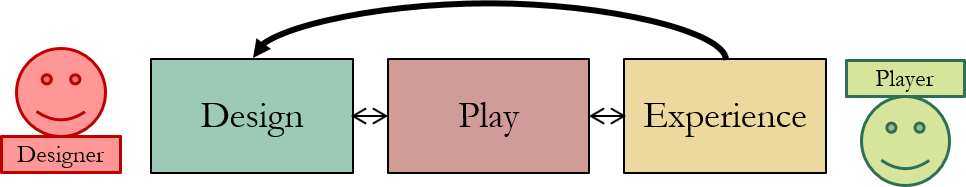
\includegraphics[width=10cm]{10_img/chap3/dpe.png} 
    \caption{Contenu des parties du Framework DPE \cite{Winn2011}}
    \label{fig.dpe}
\end{figure}

Le \gls{dpe} présenté dans la figure \ref{fig.dpe} est un framework reposant sur les mêmes principes que le MDA . Des modificatiosn sont appliquées au MDA afin d'étendre ses capacité de design pour les jeux sérieux. Il étend le framework MDA afin d'y intégrer plus facilement les notions : d'apprentissage, de  \emph{story telling}, de  \emph{gameplay} et de composants technologiques spécifiques aux jeux sérieux. Dans la figure \ref{fig.dpe_extended} sont présentés les différentes parties du DPE présenté par Winn \cite{Winn2011}.


\begin{figure}[H]
    \centering
    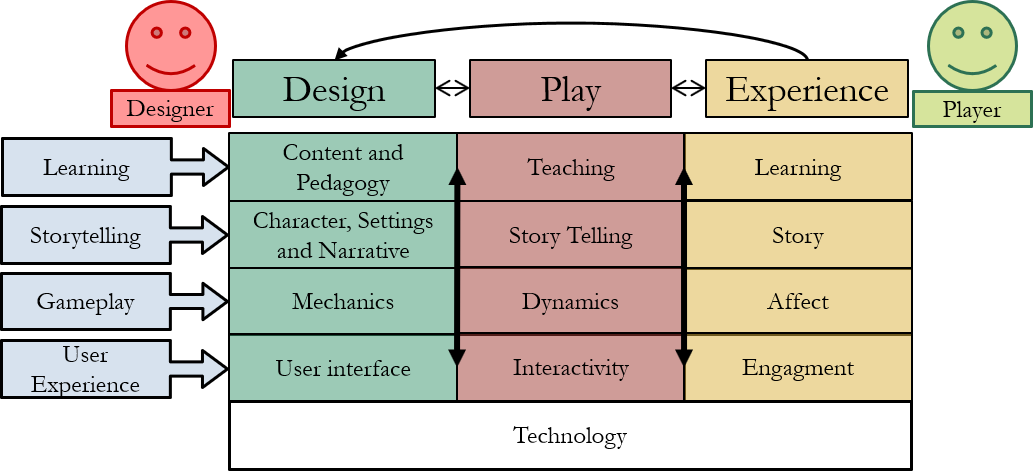
\includegraphics[width=14cm]{10_img/chap3/dpe_extended.png} 
    \caption{Framework DPE étendu \cite{Winn2011}}
    \label{fig.dpe_extended}
\end{figure}


Dans le DPE le \emph{Game Designer} a le contrôle direct sur l'ensemble des catégories. Afin d'avoir le contrôle sur la partie Expérience le \emph{Game Designer} définit des objectifs de d'Expérience. Dans la figure \ref{fig.dpe_iteratif} c'est ce qui est représenté par la flèche entre Experience et Design. Cette flèche représente également le processus itératif du design décrit par Salen et Zimmermann \cite{Salen2013}. La conception permet de produire un prototype, et l'expérience sur ce prototype permet de modifier le design afin que l'Expérience corresponde aux attentes du \emph{dame designer}.

\begin{figure}[H]
    \centering
    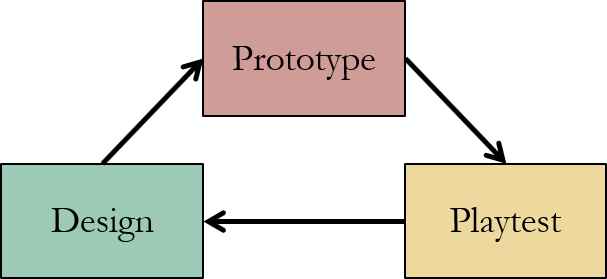
\includegraphics[width=8cm]{10_img/chap3/iteration_prototype.png} 
    \caption{Processus de design itératif \cite{Winn2011}}
    \label{fig.dpe_iteratif}
\end{figure}





\subsection{DDE : Le framework Design, Dynamics, Experience \cite{DDE}}
%ARTICLE DDE Design, Dynamics, Experience (DDE): An Advancement of the MDA framework for Game Design Wolfgang

%GAMASUTRA From MDA to DDE, Wolfgang Walk
Le framework \gls{dde} décrit dans la figure \ref{fig.dde} est présenté dans l'article de Walk et al \cite{DDE}. Ils apportent une vision critique sur le framework MDA et avancent que celui-ci néglige beaucoup d'aspects du design de jeux vidéos. Ils estiment également que le MDA se concentre trop sur les \emph{Mechanics} et ne permet donc pas de décrire tous les types de \emph{gameplay} présents sur le marché du jeu vidéo. Ce focus sur les \emph{Mechanic} entraîne, selon Walk et al, un manque de contrôle du \emph{game designer} sur les \emph{Dynamics} et \emph{Aesthetics} qui ne font que découler des \emph{Mechanics}

\begin{figure}[H]
    \begin{center}
    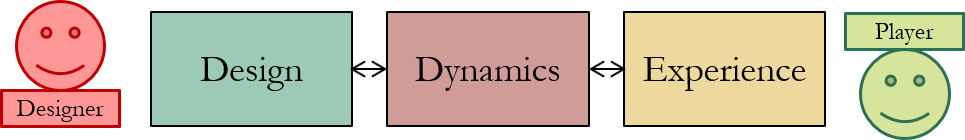
\includegraphics[width=10cm]{10_img/chap3/dde.png} 
    \caption{Contenu du Framework DDE \cite{DDE}}
    \label{fig.dde}
    \end{center}
\end{figure}

Afin de définir le framework DDE ils effectuent un découpage différent et intègrent de nouvelles notions dans les catégories comme décrits dans la figure \ref{fig.dde_extended}.

\begin{figure}[H]
    \begin{center}
    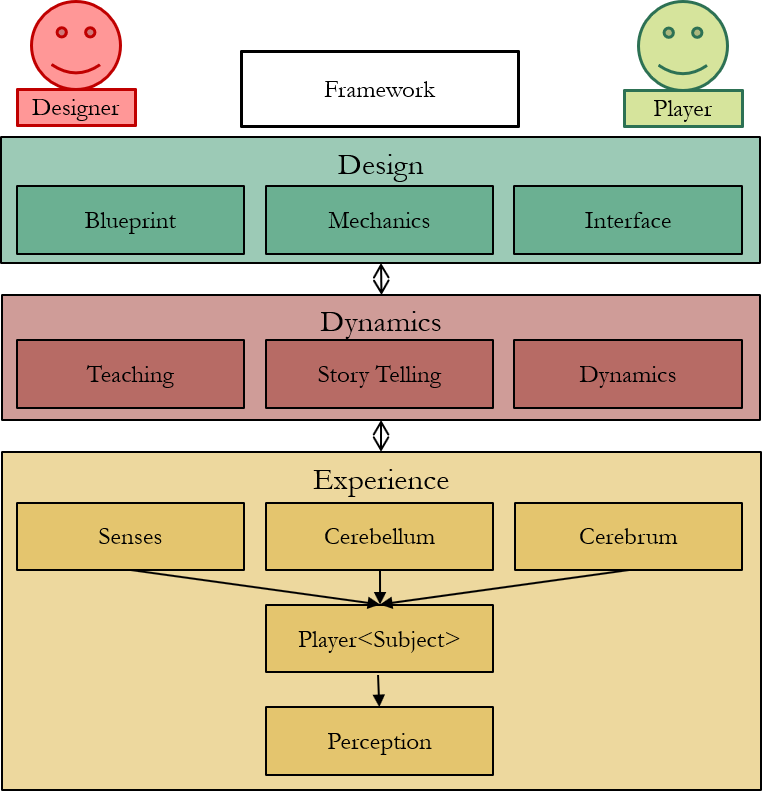
\includegraphics[width=13cm]{10_img/chap3/dde_extended_modif.png} 
    \caption{Framework DDE étendu \cite{DDE}}
    \label{fig.dde_extended}
    \end{center}
\end{figure}

\subsubsection{Design}
    \begin{itemize}
        \item \emph{Blueprint} : Partie du design qui concerne les concepts du monde du jeu : culture, religion, physique, les différents sets de règles, les styles artistiques, le design narratif, le design de personnages et le design sonore qui ensemble créés l'expérience esthétique.
        \item \emph{Mechanics} : Toute chose créant le jeu, plus précisément le code. L'architecture du code, la prise en charge des entrées/sorties, la prise en charge des objets, l'implémentation des règles de jeu et l'interaction entre les objets, et tous les éléments reliés au code. Cela comprend tous les éléments que le joueur ne perçoit pas dans son utilisation du jeu.
        \item Interface : Toutes les mécaniques qui ont pour but de communiquer le jeu au joueur. Les graphismes, le son, les réactions et interactions entre le joueur et le jeu, ainsi que celles bouclant sur le jeu lui-même. Cette partie comprend également les cinématiques les textes affichés et tout ce qu'il est possible de voir ou d'entendre dans le jeu.
    \end{itemize}

\subsubsection{\emph{Dynamics} }
    La catégorie \emph{Dynamics} du DDE correspond à celle présente dans le MDA, mais elle classifie les interactions de manière à les rendre plus précises. Cest ainsi que ces Dynamics se retrouvent en trois grande catégories: 
    \begin{itemize}
        \item Player <-> Game
        \item Player <-> Player
        \item Game <-> Game
    \end{itemize}

\subsubsection{Experience}
    Dans le MDA la troisième partie du framework est l'\emph{Aesthetics} : tout ce que le joueur sent et ressent lors de son activité sur le jeu. La partie Expérience du jeu étend l'\emph{Aesthetics} afin de prendre en considération que le joueur n'est pas une somme des émotions générées par le jeu. Le joueur devient un élément avec une expérience déjà présente avant l'utilisation du jeu ce qui peut modifier les émotions générées d'un joueur à l'autre. Une même couleur, un même son ou une même image peuvent générer différentes réactions de la part du joueur et la partie Expérience du DDE essaie de prendre en compte cela.
    \begin{itemize}
        \item Senses: expérience sensorielle du joueur du début à la fin du jeu.
        \item Cerebellum : les émotions ressenties par le joueur.
        \item Cerebrum : les challenges intellectuels et les décisions prises par le joueur.
        \item Player<Subject> : partie que le designer ne peut pas contrôler. Il peut se baser sur les trois premières catégories afin de prévoir une réponse spécifique du joueur. N'ayant aucun contrôle sur celle-ci il ne peut que estimer la réaction du joueur en fonction d'objectifs et de logiques psychologiques pour l'amener à la réaction souhaitée.
        \item Perception : ce que ressent réellement le joueur en fonction des trois première catégories et de sa propre expérience et personnalité en tant que joueur. Cela comprendra son \emph{gameplay}, le type de challenge qu'il perçoit, l'amusement qu'il ressent, la beauté qu'il perçoit, l'écho que génère l'histoire en lui, etc.
    \end{itemize}


%GAMASUTRA Revisiting the MDA framework, Luiz Claudio Silveira Duarte
\subsection{Le MDA est limités à la représentation des jeux vidéos}
Dans son article Duarte \cite{GAMA_MDA} met en avant des difficultés que le MDA a à représenter des jeux qui ne soient pas des Jeux vidéos. Il explique que les règles d'un jeu vidéo sont souvent implicites au type de \emph{gameplay} ou de genre de classification de jeu vidéos. Cependant dans le cadre des jeux de plateau les règles ne peuvent pas être implicites et acquises par l'expérience. Elles doivent être explicites et explicables dans un manuel d'utilisation. Il fait l'analogie entre un \gls{fps} et un jeu d'échecs. Dans un FPS un joueur sait à quoi s'attendre selon son expérience du genre. Il saura ou trouver les éléments et saura comment faire usage de l'interface graphique qui lui est présentée. Cependant un joueur se retrouvant devant un jeu d'échec pour la première fois ne pourra pas acquérir les connaissances requises pour jouer par l'expérience, les règles devront lui être expliquées à la base et l'expérience ne pourra lui apporter que des aspects tactiques du jeu.

\section{Conclusion}